\documentclass{article}
\usepackage[UTF8]{ctex} % Required for inserting images
\usepackage{graphicx}
\usepackage{amsmath}

\begin{document}

\section{题目3.2}

    \begin{figure}[!h]
        \centering
        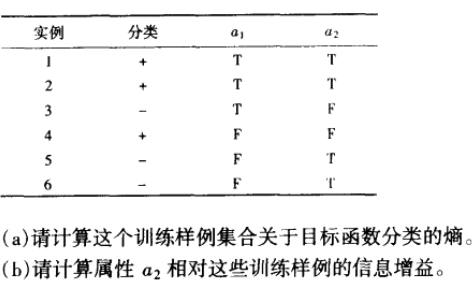
\includegraphics[width=1.2\linewidth]{image/3.2.png}
        \label{3.2}
    \end{figure}
    
    \paragraph{(a)}~{}
    
    训练样例集合有6个实例,其中3个正例(分类$+$)和3个负例(分类$-$)。  
    
    训练集熵的计算公式为:  
    \[
    \text{Entropy}(S) = -p_+ \log_2 p_+ - p_- \log_2 p_-
    \]  

    其中\(p_+\)是正例比例,\(p_-\)是负例比例。
    
    训练集中\(p_+ = 3/6 = 0.5\),\(p_- = 3/6 = 0.5\)。
    
    所以:  
    \[
    \text{Entropy}(S) = -0.5 \log_2 0.5 - 0.5 \log_2 0.5 = -0.5 \times (-1) - 0.5 \times (-1) = 0.5 + 0.5 = 1
    \]  
    
    因此,该训练样例集合关于目标函数分类的熵为1。
    

    \paragraph{(b)}~{}

    信息增益的计算公式为:  
    \[
    \text{Gain}(S, A) = \text{Entropy}(S) - \sum_{v \in \text{Values}(A)} \frac{|S_v|}{|S|} \text{Entropy}(S_v)
    \]  
    
    其中\(A\)是属性\(a_2\),有值T和F。  

    \begin{enumerate}
    \item 对于\(a_2 = T\):实例有1,2,5,6共4个实例,其中2个正例和2个负例。  
      \[
      \text{Entropy}(S_T) = - (2/4) \log_2 (2/4) - (2/4) \log_2 (2/4) = -0.5 \times (-1) - 0.5 \times (-1) = 1
      \]
      
    \item 对于\(a_2 = F\):实例有3,4共2个实例,其中1个正例和1个负例。  
      \[
      \text{Entropy}(S_F) = - (1/2) \log_2 (1/2) - (1/2) \log_2 (1/2) = -0.5 \times (-1) - 0.5 \times (-1) = 1
      \]
    \end{enumerate}

    计算信息增益:  
    \[
    \text{Gain}(S, a_2) = 1 - \left[ \frac{4}{6} \times 1 + \frac{2}{6} \times 1 \right] = 1 - \left[ \frac{6}{6} \right] = 1 - 1 = 0
    \]  
    
    所以属性\(a_2\)相对于这些训练样例的信息增益为0。


\section{题目3.3}

    \begin{figure}[!h]
        \centering
        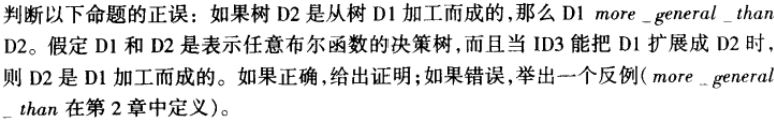
\includegraphics[width=1.2\linewidth]{image/3.3.png}
        \label{3.3}
    \end{figure}

    \paragraph{命题:}如果树D2是从树D1加工而成的,那么D1 $more\_general\_than$ D2。  
    
    该命题错误。以下是反例证明。

    \paragraph{反例:}~{}
    
    假设D1是一个简单的决策树,总是输出负例(即分类为$-$)。
    
    当D1可能是一个单节点树时,直接返回$-$。\\
    
    下面开始加工D1,添加分支条件,使得当属性\(a_1 = F\)且\(a_2 = T\)时输出正例,否则输出负例。
    
    通过对D1的加工得到D2树。\\
    
    D2的决策规则为:

    \begin{enumerate}
        \item 如果\(a_1 = F\)且\(a_2 = T\),输出$+$。
        \item 否则输出$-$。
    \end{enumerate}

    接下来比较D1和D2:

    \begin{enumerate}
        \item D1总是输出$-$,因此覆盖的正例数为0。
        \item D2在\(a_1 = F\)且\(a_2 = T\)时输出$+$,因此覆盖一些正例。
    \end{enumerate}

    根据$more\_general\_than$的定义,即“假设h1比h2更一般,当且仅当所有被h2分类为正例的实例也被h1分类为正例。“ 在上面定义的D1合D2中,当D2输出为$+$时,D1输出$-$,因此D1不覆盖D2的正例。所以D1不是$more\_general\_than$ D2。  

    又因为D2覆盖了正例,而D1没有覆盖正例,D1的正例分类为空,是D2正例分类的子集,所以D2比D1更一般,与命题矛盾。

    命题不成立,反例得证。    

\end{document}